%%
% Please see https://bitbucket.org/rivanvx/beamer/wiki/Home for obtaining beamer.
%%
\documentclass[10pt,xcolor=table]{beamer}
\usepackage[utf8]{inputenc}
%\usepackage[T2A]{fontenc}
%\usepackage[english]{babel}
\usepackage{graphicx}
\usepackage{booktabs}
\usepackage{threeparttable}
\usepackage{tikz}
\usepackage{charter}

% math
\usepackage{lmodern}
\usepackage{amsmath}
\usepackage{amssymb}
\usepackage{amsfonts}
\usepackage{mathtools}
\usepackage{bm}
\usepackage{bbm}
\newcommand\independent{\protect\mathpalette{\protect\independenT}{\perp}}
\def\independenT#1#2{\mathrel{\rlap{$#1#2$}\mkern2mu{#1#2}}}
\usepackage{amsmath}
\usepackage{amsfonts}
\usepackage{amssymb}
\DeclareMathOperator*{\argmin}{arg\,min}
\DeclareMathOperator*{\argmax}{arg\,max}
\DeclareMathOperator*{\vect}{vec}
\DeclareMathOperator\supp{supp}
\newcommand{\me}[1]{\mathbb{E} \left[ {#1} \right]}
\newcommand{\mes}[2]{\mathbb{E}_{#2} \left[ {#1} \right]}
\newcommand{\s}{\sum_{i = 1}^N}

% i don't remember what this is for
\setbeamertemplate{caption}[numbered]
\usepackage[absolute,overlay]{textpos}

%new font size
\makeatletter
\newcommand\notsotiny{\@setfontsize\notsotiny\@vipt\@viipt}
\makeatother

% for references
\usepackage{natbib}
\usepackage{apalike}

%% General slide formatting %%
\definecolor{yellow}{RGB}{242,214,0}
\definecolor{blue}{RGB}{65,105,225}

\setbeamercolor{itemize item}{fg=yellow}
\setbeamercolor{itemize subitem}{fg=blue}

%% Title slide formatting %%
%\pgfdeclareimage[width=\paperwidth]{titlebackground}{images/title-slide-background.png}
\setbeamerfont{subtitle}{size=\small}
\setbeamertemplate{title page}{
    \begin{picture}(0,0)
        \put(0,-90){%
            \begin{minipage}[b][5cm][t]{1\textwidth}
                \color{blue}
                \usebeamerfont{title}
                    {\inserttitle\\[3.5cm]} % adjust this depending on title length 
                \usebeamerfont{subtitle}
                	\color{yellow}
                    {sasha petrov  \par}
                    {\textit{3rd year}\par \vspace{1.5em}}
                    \color{blue}
                    {\insertdate \vspace{0.8em}}

            \end{minipage}
        }
    \end{picture}
}

\setbeamertemplate{headline}
{%
    \begin{picture}(0,0)
        \put(275, -28){%
            %\pgfuseimage{uchicago_logo}
        }
        \put(20,-27.5){%
            \rule{320pt}{0.4pt}
        }
    \end{picture}
}

\setbeamertemplate{frametitle}
{%
    \begin{picture}(0,0)
        \put(-8,-10){%
            \large\color{blue}\insertframetitle
        }
    \end{picture}
}

\setbeamertemplate{footline}
{%
    \begin{picture}(0,0)
        \put(20, 10){
        \notsotiny \color{yellow} sasha petrov}
        \put(150,10){% adjust this depending on text length
            \notsotiny \color{blue}\insertshorttitle
        }
        \put(337,10){%
            \notsotiny \color{yellow}\insertframenumber$/$\pageref{lastpage}
        }
    \end{picture}%
}



\setbeamertemplate{navigation symbols}{}

\title[estimating average cef derivative]{\textit{Model selection for estimating CEF derivatives}}


\begin{document}
\setbeamercovered{transparent}


\begin{frame}[plain]
    \titlepage
\end{frame}

\begin{frame}{Fixing objects}

From the \textit{all causes} framework, the object of interest:

	\begin{equation}
	\left\{ \frac{\partial}{\partial x} \phi(X, u) \right\}_{u \in supp \, U}
\end{equation}

The average that's considered to be a more feasible target:

\begin{equation}
	\frac{\partial}{\partial x} \mathbb{E} \left[ \phi(X, U) | X = x \right]
\end{equation}

Weight derivatives at different values of the domain with the density of those values:

\begin{equation}
	\mathbb{E} \left[ \frac{\partial}{\partial x} \mathbb{E} \left[ \phi(X, U) | X = x \right] \right]
\end{equation}


\end{frame}

\begin{frame}{Can we do model selection in this context -- 1}
	Even if you have a decent predictor for levels $\hat f(x)$, it might not work as well for predicting $f(x') - f(x)$. Think of the average treatment effect as a result of moving from $x$ to $x'$.
	
	\begin{itemize}
		\item Recall Yitzhaki weights -- $\beta_{BLP}$ estimates a `weird' average of derivatives with weights
		\item Banerjee (2007): Directly target the average derivative -- local OLS is offered as a solution
	\end{itemize}
	
To me this looks like a b/v issue but with an interesting twist -- both supervised and unsupervised ?? How much can we gain in terms of variance by imposing the bias of the sort that $\beta_{BLP}$ does?

What could do for the proj with reasonable prob: Take a context, simulate (wiemann style) and see if BLP can do better for some dgps?
\end{frame}

\begin{frame}{Can we do model selection in this context -- 2}
	\begin{itemize}
		\item What is the bias like for $\beta_{BLP}$ in this setting? Can we obtain the parameter that $\beta_{BLP}$ estimates as a result of some penalisation? So it would be a penalisation that leads to the bandwidth being the complete domain, right?
		\item When we do lasso: we chose a particular `space' with respect to which to penalise the model, right? What can we choose as a `space' in this case of estimating derivatives?
		\item It seems weird to impose a minimum distance between the set of weights and the pdf of $X$, right? Maybe penalise directly the distance between the set of Yitzhaki weights and the true pdf of $X$?
	\end{itemize}
	
	Set of weights $\omega: supp \, X \rightarrow \mathbf{R}_+$.

\begin{align}
	\min d(\omega, f_X) \\
	\textrm{s.t.} \, d(\omega, \omega_z) \leq \lambda
\end{align}
\end{frame}


\begin{frame}{monte carlo}
\begin{equation}
\begin{split}
X \sim U [0, 1] ^ n \\
\varepsilon \sim \mathcal{N} (0, 1) \quad X \perp \varepsilon \\
Y = X ^ 2 + \varepsilon
\end{split}
\end{equation}

Average derivative: $1$


\end{frame}


\begin{frame}{ridge / rkhs}

Vapnik kernel:

\begin{equation}
  J[f] = \s \left( y_i - f(x_i) \right)^2 + \lambda || f ||^2_{\mathcal{H}}
\end{equation}


\begin{equation}
K(x, y) = 1 + 2 x y + x^2 y^2
\end{equation}

\end{frame}


\begin{frame}{average derivative vs mse}
	\begin{figure}[ht]
        \begin{minipage}[t]{0.45\linewidth}
            \centering
            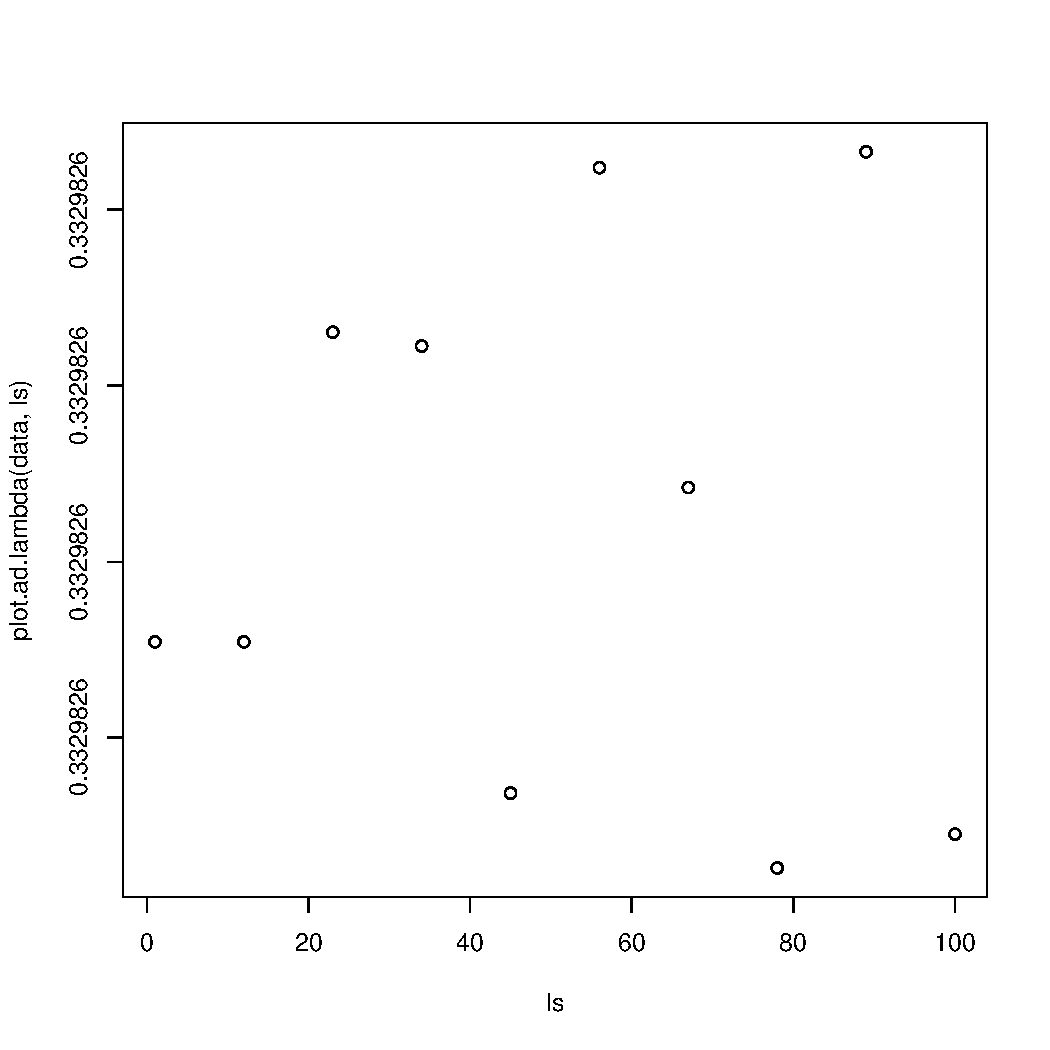
\includegraphics[width = \textwidth, keepaspectratio]{ad_lambdas.pdf}
                       \caption{deviation from average derivative}
            \label{fig:a}
        \end{minipage}
        \hspace{0.5cm}
        \begin{minipage}[t]{0.45\linewidth}
            \centering
            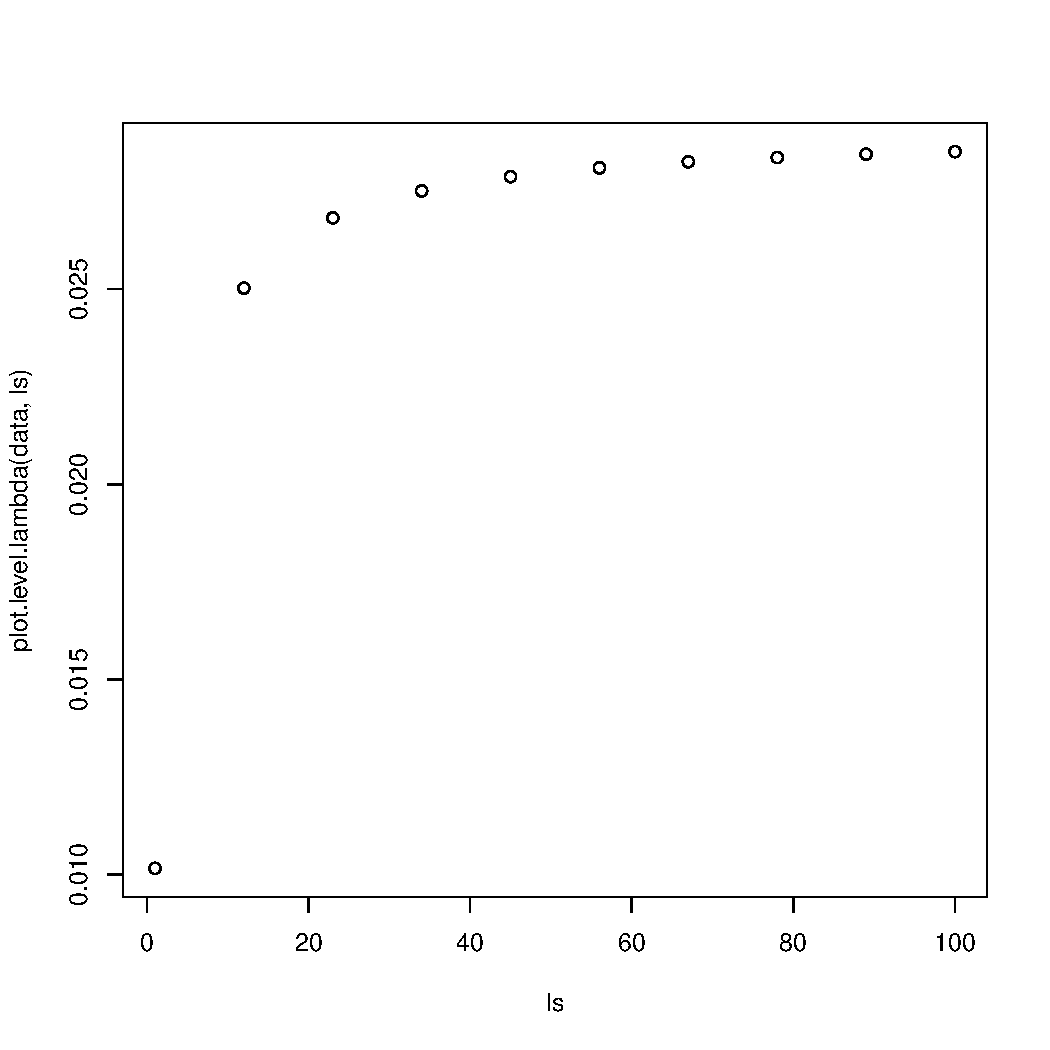
\includegraphics[width = \textwidth, keepaspectratio]{mse_lambdas.pdf}
                        \caption{mse}
            \label{fig:b}
        \end{minipage}
    \end{figure}
\end{frame}


\begin{frame}{using yitzhaki weights}
	choose $\lambda$ based on the distance between yitzhaki weights and the true density
\end{frame}


\begin{frame}{kl distance as a function of the power}
\begin{center}
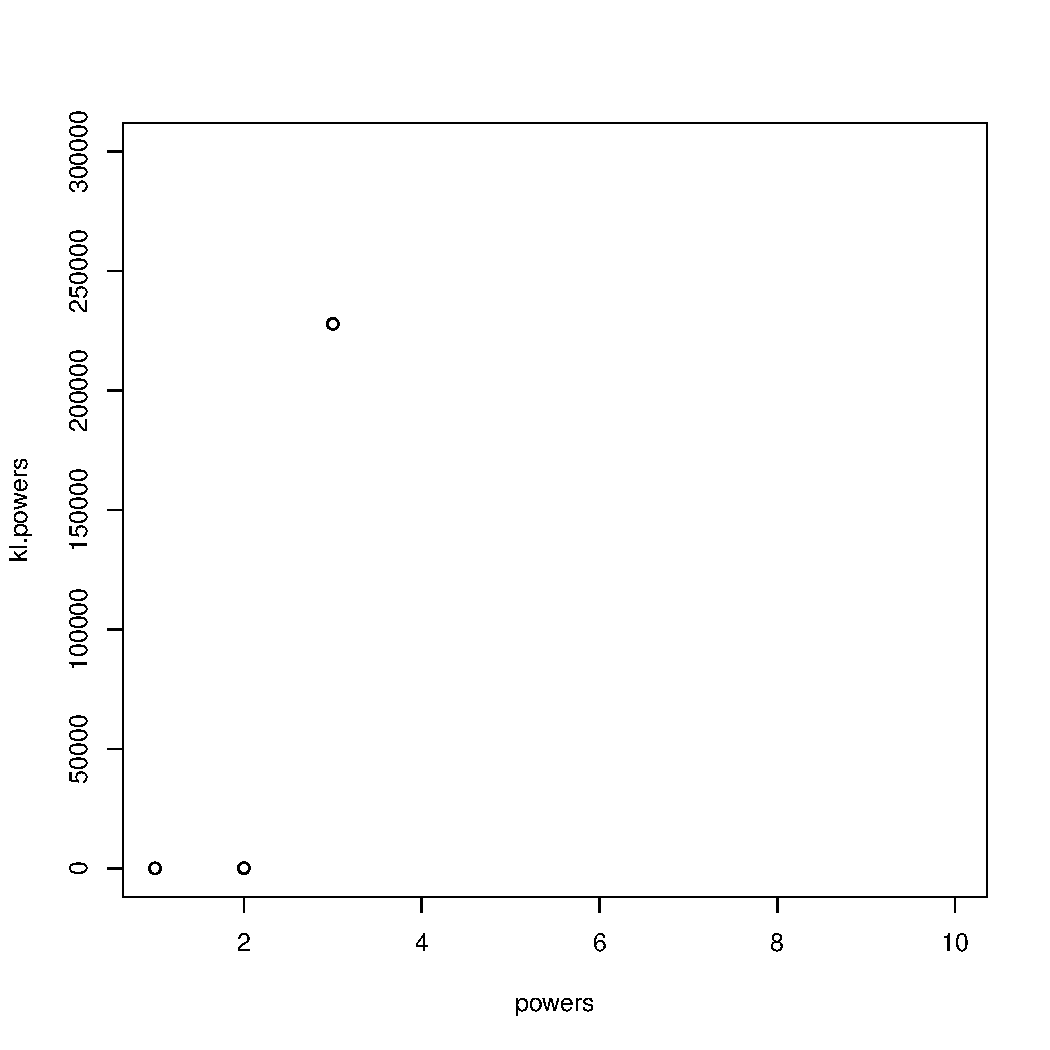
\includegraphics[width=0.8\textwidth,keepaspectratio]{kl.pdf}
\end{center}
\end{frame}

%% References
\begin{frame}{References} 
\label{lastpage} \small % adjust size if needed
\bibliographystyle{apalike}
%\bibliography{biblio}
\end{frame}


\end{document}